\section{Принятие решения на вылет и выбор запасных аэродромов}


\subsection{Общие правила}


\paragraph{} КВС принимает решение на вылет на основании:
\begin{itemize}
    \item готовности экипажа к выполнению полета;
    \item технической готовности ВС;
    \item анализа метеообстановки;
    \item анализа воздушной обстановки и обеспечения полета;
    \item анализа адекватности аэродромов вылета, назначения и запасных, включая анализ:
    \begin{itemize}
        \item состояния летного поля, ВПП, рулежных дорожек, перронов;
        \item наличия и работоспособности навигационных средств, состояния светотехнического оборудования;
        \item обеспечения требуемого эксплуатационного минимума для посадки;
        \item наличия ограничений, запретов на выполнение полетов, необходимости предварительного запроса;
        \item соответствия категории аэродрома по уровню требуемой пожарной защиты типу ВС.
    \end{itemize}
\end{itemize}

\paragraph{} Командиру ВС разрешается выбирать для взлета и посадки на самолете площадку, о которой отсутствует аэронавигационная информация, если она осмотрена с земли или подобрана с воздуха и признана командиром ВС удовлетворяющей требованиям РЛЭ ВС. Для допуска к посадкам на площадку, подобранную с воздуха, пилот самолета должен пройти соответствующую подготовку под руководством инструктора.
Коммерческие перевозки пассажиров на самолетах с подбором площадок с воздуха запрещены.

\chgdPar{xx.xx.xx}{34}{Если при подготовке к полету оказалось, что взлетная масса воздушного судна превышает допустимую для фактических условий на старте, командир ВС имеет право принять решение о переносе вылета или снятии части груза.}

Если метеоусловия на аэродромах вылета, назначения и (или) запасных, а также по маршруту в период между первоначальным получением метеорологической информации для принятия решения на вылет и вылетом ВС по информации диспетчера ОВД ухудшились и не соответствуют правилам принятия решения на вылет, командир ВС в этом случае обязан пересмотреть решение на вылет.

При задержке более чем на 20 минут от времени вылета, предусмотренного планом полета, командир воздушного судна обязан получить повторное разрешение на вылет. Метеоинформацию и повторное разрешение на вылет разрешается получать по радио (другим средствам связи).

В случае задержки на 30 мин. и более после расчетного времени начала выполнения контролируемого полета или на 1 час и более начала неконтролируемого полета план полета должен быть изменен или представлен новый план полета. Командир ВС обязан повторно принять решение на вылет.

\paragraph{} Принятие решения на вылет, взлет и посадку воздушного судна производится по наивысшему из установленных минимумов:  
\begin{itemize}
    \item командира воздушного судна (минимума, указанного в задании на полет; при принятии решения по минимуму КВС ниже CAT I, необходимо наличие допуска к таким заходам на посадку у остальных членов экипажа);
    \item аэродрома (эксплуатационного);
    \item воздушного судна.
\end{itemize}

При принятии решения на выполнение взлета (посадки) соответствие фактического ветра установленным ограничениям определяется с учетом его порывов.

Командиру ВС, выполняющему международные рейсы, разрешается принимать самостоятельное решение на продолжение рейса в случаях задержек в иностранных аэропортах с учетом того, чтобы общее рабочее время не превышало установленных норм рабочего времени и, находясь в контакте с представителем Авиакомпании, диспетчером ОКВР, принимать меры по сокращению возможных задержек.

\subsection{Выбор запасных аэродромов при вылете}

\paragraph{} \label{par:altrule2} Для самолетов запасной аэродром при взлете должен выбиратЬся и указыватЬся в рабочем плане полета в тех случаях, когда метеорологические условия на аэродроме вылета равны установленному эксплуатационному минимуму аэродрома для посадки, который может быть применен, или ниже его, или не представляется возможным вернуться на аэродром вылета по другим причинам. 

Для самолетов запасной аэродром при взлете выбирается в пределах следующего расстояния от аэродрома вылета при расчете в стандартных атмосферных условиях, в штиль, с использованием фактической взлетной массы:
\begin{itemize}
    \item для самолетов с двумя силовыми установками - не дальше расстояния, эквивалентного одному часу времени полета на крейсерской скорости с одним неработающим двигателем, определенном в соответствии с РЛЭ ВС (AFM, FCOM) или установленному эксплуатантом времени, но не более 2-х часов полета, если эксплуатант имеет разрешение на полеты по правилам EDTO не менее 120 минут;
    \item для самолетов с тремя или более силовыми установками - не дальше расстояния, эквивалентного 2-м часам времени полета на крейсерской скорости с одним неработающим двигателем.
\end{itemize} 

Запасной аэродром для взлета выбирается при соответствии фактической погоды или прогноза погоды эксплуатационному минимуму аэродрома для посадки, который может быть применен в течение периода времени, начинающегося за 1 час до и заканчивающегося через 1 час после расчетного времени прибытия с учетом ограничений в случае отказа одного двигателя. 

\paragraph{} \label{par:altrule} Кроме случаев, указанных в «Руководстве по выполнению полетов по правилам EDTO», выбирается пригодный для посадки запасной аэродром по маршруту следования таким образом, чтобы с любой точки маршрута до выбранного запасного аэродрома на маршруте время полета с одним отказавшим двигателем в стандартной атмосфере в штиль не превышало 60 минут для ВС с двумя газотурбинными двигателями или 180 минут с тремя и более двигателями.

Запасные аэродромы на маршруте указываются в рабочем плане полета.

\paragraph{} В качестве пригодного для посадки может использоваться аэродром, на котором;
\begin{itemize}
    \item посадочные характеристики ВС позволяют выполнить безопасную посадку;
    \item имеются светотехническое оборудование и средства связи;
    \item имеются метеорологическое и аварийно-спасательное обеспечение, навигационные средства;
    \item имеется хотя бы одна схема захода на посадку по приборам;
    \item имеются необходимые виды и средства обслуживания, соответствующие техническим характеристикам воздушного судна и который находится в рабочем состоянии в ожидаемое время использования.
\end{itemize}


\begin{enumerate}[label=\arabic*),ref=\arabic*]
    \item посадочные характеристики ВС позволяют выполнить безопасную посадку;
    \item имеются светотехническое оборудование и средства связи;
    \item имеются метеорологическое и аварийно-спасательное обеспечение, навигационные средства;
    \item имеется хотя бы одна схема захода на посадку по приборам;
    \item имеются необходимые виды и средства обслуживания, соответствующие техническим характеристикам воздушного судна и который находится в рабочем состоянии в ожидаемое время использования.
    
\end{enumerate}

\begin{enumerate}
    \item посадочные характеристики ВС позволяют выполнить безопасную посадку;
    \item имеются светотехническое оборудование и средства связи;
    \item имеются метеорологическое и аварийно-спасательное обеспечение, навигационные средства;
    \item имеется хотя бы одна схема захода на посадку по приборам;
    \item имеются необходимые виды и средства обслуживания, соответствующие техническим характеристикам воздушного судна и который находится в рабочем состоянии в ожидаемое время использования.    
\end{enumerate}

\begin{enumerate}[label=\alph*),ref=\alph*]
    \item посадочные характеристики ВС позволяют выполнить безопасную посадку;
    \item имеются светотехническое оборудование и средства связи;
    \item имеются метеорологическое и аварийно-спасательное обеспечение, навигационные средства;
    \item имеется хотя бы одна схема захода на посадку по приборам;
    \item имеются необходимые виды и средства обслуживания, соответствующие техническим характеристикам воздушного судна и который находится в рабочем состоянии в ожидаемое время использования.    
\end{enumerate}

\begin{enumerate}[label=\asbuk*),ref=\asbuk*]
    \item посадочные характеристики ВС позволяют выполнить безопасную посадку;
    \item имеются светотехническое оборудование и средства связи;
    \item имеются метеорологическое и аварийно-спасательное обеспечение, навигационные средства;
    \begin{itemize}
        \item посадочные характеристики ВС позволяют выполнить безопасную посадку;
        \item имеются светотехническое оборудование и средства связи;
        \item имеются метеорологическое и аварийно-спасательное обеспечение, навигационные средства;
        \item имеется хотя бы одна схема захода на посадку по приборам;
        \item имеются необходимые виды и средства обслуживания, соответствующие техническим характеристикам воздушного судна и который находится в рабочем состоянии в ожидаемое время использования.
    \end{itemize}
    \item имеется хотя бы одна схема захода на посадку по приборам;
    \item имеются необходимые виды и средства обслуживания, соответствующие техническим характеристикам воздушного судна и который находится в рабочем состоянии в ожидаемое время использования.    
\end{enumerate}

Запасной аэродром должен находиться в рабочем состоянии в ожидаемое время использования.

Запасными аэродромами на маршруте могут быть аэродромы вылета и пункта назначения.

Запасной аэродром по маршруту (3\% ERA) - подходящий аэродром по маршруту, который может потребоваться на этапе планирования, выбранный в целях снижения до 3\% Route Reserve на случай непредвиденных обстоятельств.

Особенности расположения «3\%-го» запасного аэродрома по маршруту (3\% ERA) для уменьшения Route Reserve до 3\% описаны в \hyperref[par:497]{пункте \ref*{par:497}} настоящей главы.


\begin{table}[H]
    \begin{center}
    \caption{Зона оперирования ВС при выборе запасных аэродромов для взлета и по маршруту} \label{tbl:altto}
    \begin{tabular}{|p{0.20\textwidth}|p{0.32\textwidth}|p{0.32\textwidth}|}
    \hline
    &\multicolumn{2}{c|}{Максимальное время полета до запасного аэродрома}\\
    \cline{2-3}
    Тип ВС&\multicolumn{2}{c|}{60 минут}\\
    \cline{2-3}
    &Для взлета&Маршрут\\
    \hline
    Ан-24/26	&330км	&330км\\
    \hline
    Ан-74	    &400км	&400км\\
    \hline\hline


    \end{tabular}
    \end{center}
\end{table}

\textbf{Примечание:} \textit{Указанные в таблице границы зоны оперирования и скорости ВС используются только на этапе планирования полета для построения маршрута и не являются эксплуатационным ограничением при выполнении ухода на пригодный для посадки аэродром. В зависимости от крейсерского эшелона полета и ряда других факторов фактическое время полета при уходе на запасной аэродром может превышать установленное максимальное время полета до запасного аэродрома.}

\paragraph{}{Выбор запасного аэродрома пункта назначения}\label{sect:alt}

При полете по ППП выбирается и указывается в планах полета, по крайней мере, один запасной аэродром пункта назначения, уход на который возможен с ВПР аэродрома назначения или с заранее запланированной точки на маршруте (рубежа ухода), за исключением случаев, когда продолжительность полета не превышает 6 часов, аэродром назначения имеет две независимые ВПП, пригодные для посадки ВС, и получена информация о фактической, прогнозируемой погоде, дающая уверенность в том, что в течение периода времени, начинающегося за 1 час до и заканчивающегося через 1 час после расчетного времени прибытия, видимость будет не менее 5000м, а нижняя граница облаков (вертикальная видимость) будет не ниже 600м и превышать MDH для захода на посадку с применением визуального маневрирования («circle-to-land») не менее чем на 150 м, а в случае, если такая высота не опубликована, то не ниже безопасной высоты в районе аэродрома (секторе захода на посадку).

В качестве запасного аэродрома пункта назначения может использоваться аэродром пункта назначения при наличии двух независимых ВПП.
Примечание. Независимыми ВПП являются две или более ВПП на том же самом аэродроме, расположенные таким образом, что если одна ВПП закрыта, то производство полетов можно обеспечивать с помощью другой.

\paragraph{} \label{par:alt0}При расчетной продолжительности полета с рубежа ухода до аэродрома назначения более 2 часов информация о фактической и прогнозируемой погоде на аэродроме назначения должна указывать на то, что в течение периода времени, начинающегося за 2 часа до и заканчивающегося через 2 часа после расчетного времени прибытия, нижняя граница облаков (вертикальная видимость) и видимость будут соответствовать требованиям настоящего раздела, но не ниже 200 м и не менее 2500 м соответственно.

\paragraph{} \label{par:alt1}За исключением случаев, указанных в \hyperref[par:alt2]{пункте \ref*{par:alt2}}  настоящего раздела, полет по ППП не начинается до тех пор, пока КВС не будет получена информация, указывающая на то, что:
\begin{itemize}
    \item условия на аэродроме намеченной посадки к расчетному времени прилета будут соответствовать эксплуатационному минимуму аэродрома или превышать их;
    \item условия на запасном аэродроме пункта назначения, если таковой требуется, к расчетному времени прилета будут соответствовать при планируемом заходе на посадку:
    \begin{itemize}
        \item по САТ II и/или III* - нижней границе облаков (вертикальной видимости) не ниже 60 м, видимости (RVR) - не менее эксплуатационного минимума аэродрома для посадки при САТ I;
        \item по радиомаячным системам инструментального захода на посадку (кроме САТ II и/или III*) – нижней границе облаков (вертикальной видимости) не ниже MDH для захода по схеме неточного захода на посадку, видимости(RVR)-не менее эксплуатационного минимума захода по схеме неточного захода на посадку;
        \item при заходе по схеме неточного захода на посадку-нижней границе облаков (вертикальной видимости) превышающей MDH для захода по схеме неточного захода на посадку не менее чем на 50м, видимости (видимости на ВПП) – превышающей эксплуатационный минимум для посадки при выполнении захода по схеме неточного захода на посадку не менее чем на 500 м;
        \item с применением визуального маневрирования («circle-to-land») - нижней границе облаков (вертикальной видимости) превышающей MDH для захода на посадку с применением визуального маневрирования не менее чем на 100 м, видимости, превышающей эксплуатационный минимум для захода на посадку с применением визуального маневрирования не менее чем на 1000 м.
    \end{itemize}
\end{itemize}

\paragraph{} \label{par:alt2}При отсутствии информации о метеорологических условиях (МУ) аэродрома назначения или при наличии информации, свидетельствующей о погоде ниже минимума для посадки к расчетному времени прибытия, выбираются два запасных аэродрома пункта назначения с МУ, соответствующими требованиям \hyperref[par:alt1]{пункта \ref*{par:alt1}}  настоящего раздела РПП, или один запасной аэродром, на котором видимость будет не менее 5000 м, а нижняя граница облаков (вертикальная видимость) будет не ниже 450 м. и превышать MDH для захода на посадку с применением визуального маневрирования не менее чем на 150м, а если такая высота не опубликована, то не ниже БВП в районе аэродрома (в секторе захода на посадку).

В качестве указанной информации используются сведения, полученные от полномочного метеорологического органа, которые Авиакомпания признает достоверными.

При выборе запасных аэродромов используются эксплуатационные минимумы аэродрома для посадки, применимые для конкретной ВПП с учетом направления и скорости ветра.

Аэродром вылета может быть запасным аэродромом для взлета, на маршруте или для аэродрома назначения для вылетающего воздушного судна.

\paragraph{} На изолированные аэродромы Авиакомпания полеты не выполняет

\subsection{Правила определения пригодности аэродрома}

\paragraph{} При определении пригодности аэродрома учитывается:
\begin{itemize}
    \item характеристики аэродрома (расположение, превышение, климатические характеристики, характеристики ВПП, РД, перронов и т.п.);
    \item несущая способность искусственного покрытия ВПП путем определения соответствия классификационного числа покрытия (англ. Pavement Classification Number (PCN)) и классификационного числа ВС (англ. Aircraft Classification Number (ACN)), если ограничения аэродрома не публикуют дополнительную информацию;
    \item наличие достаточного объема действующей аэронавигационной информации по данному аэродрому;
    \item ограничения по выполнению полетов, включая ограничения по шуму, установленные на данном аэродроме;
    \item уровень обеспечения средствами спасания и пожарной защиты;
    \item наличие требуемых видов обеспечения полетов ВС и организации воздушного движения на данном аэродроме для эксплуатируемого типа ВС и вида выполняемых полетов.
\end{itemize}


\paragraph{} Оценка состояния покрытия ВПП и показатели эффективности торможения.

Оценка состояния элементов летного поля производится по значениям величин, получаемых в процессе измерений, параметров оценки.

К параметрам оценки состояния покрытий относятся:
\begin{itemize}
    \item фрикционные свойства покрытий;
    \item вид осадков;
    \item толщина слоя осадков;
    \item доля площади, покрытая загрязнениями.
\end{itemize}


Фрикционные (тормозные) свойства покрытий оцениваются величиной коэффициента сцепления.

Вид осадков оценивается кодовыми цифрами от 1 до 9, с соответствующей каждому числу описательной характеристикой осадков. 
Толщина слоя осадков оценивается числом, соответствующим толщине слоя в миллиметрах. Доля площади, покрытая осадками, оценивается в процентах.

Коэффициент сцепления, в зависимости от применяемых средств, определяется непосредственным отсчетом результатов измерений (\hyperref[tbl:04T2]{Таблица \ref*{tbl:04T2}}), либо приведением результатов измерений к нормативным значениям с помощью корреляционных зависимостей (\hyperref[tbl:04T3]{Таблица \ref*{tbl:04T3}})\footnote{Таблицы могут быть где угодно}.

Значения нормативного коэффициента сцепления отражают относительное улучшение или ухудшение эффективности торможения.
При отсутствии в аэропорту инструментальных средств оценки фрикционных средств дается расчетная эффективность торможения - кодовая оценка состояния покрытия ВПП (\hyperref[tbl:04T2]{Таблица \ref*{tbl:04T2}}).

\begin{table}[]
    \begin{center}
    \caption{Расчетная эффективность торможения} \label{tbl:04T2}
    \small
    \begin{tabular}{|p{0.07\textwidth}|p{0.20\textwidth}|p{0.25\textwidth}|p{0.37\textwidth}|}
    \hline
    Код	&Измеренный коэффициент сцепления	&Расчетная эффективность торможения	&Эксплуатационные ограничения\\
    \hline
    5	&0.60 - 0.40	                    &Хорошая	                        &Отсутствие затруднений по путевому управлению\\
    4	&0.39 - 0.36	                    &Средняя хорошая	                &Отсутствие затруднений по путевому управлению\\
    3	&0.35 - 0.30	                    &Средняя	                        &Возможно ухудшение путевого управления\\
    2	&0.29 - 0.26	                    &Средняя плохая	                    &Возможно ухудшение путевого управления\\
    1	&0.25 - 0.18	                    &Плохая	                            &Путевое управление будет плохим\\
    9	&0.17 и ниже	                    &Ненадежная	                        &Путевое управление не контролируется\\
    \hline\hline
    \end{tabular}
    \end{center}
\end{table}

\begin{table}[]
    \begin{center}
    \caption{} \label{tbl:04T3}
    \small
    \begin{tabular}{|p{0.20\textwidth}|p{0.25\textwidth}|p{0.37\textwidth}|}
    \hline
    Нормативный коэффициент сцепления	&Расчетная эффективность торможения	&Эксплуатационные ограничения\\
    \hline    
    0.57 - 0.42	                        &Хорошая	                        &Отсутствие затруднений по путевому управлению\\
    0.41 - 0.40	                        &Средняя хорошая	                &Отсутствие затруднений по путевому управлению\\
    0.39 - 0.37	                        &Средняя	                        &Возможно ухудшение путевого управления\\
    0.36 - 0.35	                        &Средняя плохая	                    &Возможно ухудшение путевого управления\\
    0.34 - 0.30	                        &Плохая	                            &Путевое управление будет плохим\\
    0.29 и ниже	                        &Ненадежная	                        &Путевое управление не контролируется\\        \hline\hline
    \end{tabular}
    \end{center}
\end{table}


\paragraph{} Оценка состояния покрытия по описательной характеристике 

Кодовая оценка состояния покрытия ВПП составляется на основании субъективного опыта лица, выполняющего оценку. Для составления кодовой оценки справочно может использоваться таблица соответствия нормативного коэффициента сцепления описательной характеристике состояния покрытия (\hyperref[tbl:04T4]{Таблица \ref*{tbl:04T4}}). 

\begin{table}[H]
    \begin{center}
    \caption{Таблица соответствия нормативного коэффициента сцепления описательной характеристике состояния покрытия} \label{tbl:04T4}
    \small
    \begin{tabular}{|p{0.40\textwidth}|p{0.20\textwidth}|}
    \hline
    Описательная характеристика состояния поверхности	&Нормативный коэффициент сцепления\\
    \hline    
    Сухой цементобетон или асфальтобетон	            &0,6 и выше\\
    Влажный цементнобетон или асфальт	                &0,4 - 0,6\\
    Мокрый асфальтобетон	                            &0,3 - 0,6\\
    Асфальтобетон, местами лужи	                        &0,28 - 0,4\\
    Уплотненный снег при t ниже- 15°C	                &0,3 - 0,5\\
    Уплотненный снег при t выше - 14°C	                &0,2 - 0,25\\
    Лед при t выше - 10°C	                            &0,1 - 0,2\\
    Лед тающий	                                        &0,05 - 0,1\\
    \hline\hline
    \end{tabular}
    \end{center}
\end{table}

\begin{description}
    \item[Влажно] соответствует состоянию, когда поверхность изменяет цвет вследствие наличия влаги.
    \item[Мокро] поверхность пропитана водой, но стоячая вода отсутствует. 
    \item[Участки воды] видны участки стоячей воды.
    \item[Иней или изморозь] снеговидные кристаллические льдообразования на поверхности покрытия, образующиеся, как правило, в утренние часы и связанные с охлаждением поверхности. 
    \item[Сухой снег] снег, который будучи в рыхлом состоянии может сдуваться ветром или рассыпаться; плотность – до 0,35, но, не включая 0,35.
    \item[Мокрый снег] снег, который не рассыпается и образует или имеет тенденцию образовывать снежный ком; плотность - от 0,35 и до, но, не включая 0,5.
    \item[Слякоть] пропитанный водой снег, который при ударе разбрызгивается в стороны; плотность от 0,5 до 0,8.
    \item[Лед] вода в замерзшем состоянии, на аэродромных покрытиях проявляется в виде гололеда или гололедицы.
\end{description}

\textbf{Предупреждение! Посадка и взлет ВС на аэродромах Российской Федерации при нормативном Ксц менее 0,3 запрещаются.}

\paragraph{}Определение соответствия категории аэродрома по уровню обеспечения средствами спасения и пожарной защиты типу ВС



Категория аэродрома по организации аварийного обслуживания (Emergency services, Rescue and Fire Fighting) определяется в соответствии с классификацией ICAO требуемому уровню средств спасения и пожарной защиты, который обеспечивается на аэродроме для наибольшего по размерам (длине и ширине фюзеляжа) типа ВС, выполняющего полеты на данный аэродром.

Информация о категории аэродрома публикуется в сборниках аэронавигационной информации и NОТАМ.

Обеспечиваемый уровень средств спасения и пожарной защиты (ССПЗ) на аэродромах вылета и назначения в стандартных условиях должен быть не ниже уровня требуемой пожарной защиты (УТПЗ) для данного типа ВС (см. \hyperref[tbl:04T5]{таблицу \ref*{tbl:04T5}}).



\begin{table}[H]
    \begin{center}
    \caption{Требуемый УТПЗ} \label{tbl:04T5}
    \small
    \begin{tabular}{|p{0.25\textwidth}|p{0.08\textwidth}|p{0.08\textwidth}|p{0.08\textwidth}|p{0.08\textwidth}|}
    \hline
    Категория аэродрома  &\multicolumn{4}{c|}{Типы ВС} \\
    \cline{2-5}
    по УТПЗ                     &Ан-2   &Ан-24/26   &Ан-74  &CL300\\
    \hline    
    1                           &       &  ЗОНА II  &       &       \\\hline
    2                           &       &           &ЗОНА II&ЗОНА II\\\hline
    3                           &x      &           &       &       \\\hline
    4                           &       &x          &       &       \\\hline
    5                           &Зона I &           &x      &x      \\\hline
    6                           &       &Зона I     &       &       \\\hline
    7                           &       &           &Зона I &Зона I \\
    \hline\hline
    \end{tabular}
    \end{center}
\end{table}
Х – нормальный для типа ВС УТПЗ

Категория ВПП по УТПЗ может быть понижена на одну ступень относительно величины, определенной по длине и максимальной ширине фюзеляжа, если на аэродроме количество взлетов или посадок наибольшего для данной ВПП ВС менее 700 для трех самых интенсивных по полетам месяцев года.

В случае временного уменьшения, требуемого для данного типа ВС уровня УТПЗ на аэродроме вылета и назначения, при принятии решения на полет следует руководствоваться следующими положениями:
\begin{itemize}
    \item если УТПЗ на аэродроме снизился не более чем на 2 единицы от требуемого для данного типа воздушного судна - полет может быть выполнен без ограничений;
    \item если УТПЗ на аэродроме снизился более чем на 2 единицы от требуемого для данного типа ВС - полет может быть выполнен по согласованию с администрацией аэропорта и руководством авиакомпании, принимая во внимание имеющуюся информацию о фактическом положении дел относительно обеспеченности данного аэродрома.
\end{itemize}

	
Для запасных аэродромов значение УТПЗ не может быть снижен более чем на 3 единицы от требуемого уровня для данного типа ВС. 

Если информация о снижении уровня УТПЗ на аэродроме получена в полете, для принятия решения экипаж должен руководствоваться \hyperref[tbl:04T6]{таблицей \ref*{tbl:04T6}} 

 
\begin{table}[H]
    \begin{center}
    \caption{} \label{tbl:04T6}
    \small
    \begin{tabular}{|p{0.08\textwidth}|p{0.85\textwidth}|}
    \hline
    ЗОНА I  &продолжить полет до аэродрома назначения;\\\hline
    ЗОНА II &продолжить полет до аэродрома назначения, но не начинать заход на посадку пока не будет получено подтверждение от администрации аэродрома, что все имеющиеся на аэродроме ресурсы ССПЗ подготовлены для применения в районе ВПП, планируемой для посадки ВС;\\\hline
    ЗОНА III&следовать на запасной аэродром в случае, если КВС считает, что уход на запасной более безопасен, чем посадка на а/д назначения. Если КВС принято решение о посадке на а/д назначения, то должны быть выполнены положения, определенные для ЗОНЫ II – имеющиеся ресурсы ССПЗ подготовлены для применения в районе ВПП, планируемой для посадки ВС.\\
    \hline\hline
    \end{tabular}
    \end{center}
\end{table}

	

\subsection{Принятие решения на вылет по ППП}

\paragraph{}Командир ВС принимает решение на вылет по ППП на основании анализа метеорологической обстановки, если:
\begin{itemize}
    \item на аэродроме вылета фактическая погода не ниже минимума, установленного для взлета.
    
    В том случае, если метеорологические условия на аэродроме вылета равны установленным эксплуатационным минимумам аэродрома для посадки или ниже их или не представляется возможным вернуться на аэродром вылета по другим причинам, необходимо выбрать запасной аэродром для взлета в соответствии с \hyperref[par:altrule2]{п. \ref*{par:altrule2}}; 
    \item на маршруте полета отсутствуют опасные метеоявления, обход которых невозможен;
    \item на аэродроме намеченной посадки фактическая погода и прогнозируемые условия погоды ко времени прилёта соответствуют требованиям одного из вариантов Таблицы А8.4-Т7 при принятии решения на вылет на аэродромы, где установлен государственный минимум и на которых совместно со значениями MDH(DH) дополнительно представлена информация о минимальном значении НГО в таблице минимумов с пометкой «CEILING REQUIRED» применять наибольшее из опубликованных значений MDH (DH) или НГО за параметр выбранного минимума для посадки;
    \item имеются запасные аэродромы по маршруту, выбранные в соответствии с \hyperref[par:altrule]{п. \ref*{par:altrule}}  и имеются запасные аэродромы для аэродрома назначения, в соответствии с \hyperref[sect:alt]{п. \ref*{sect:alt}}, с исключениями, указанными в \hyperref[par:altex]{п. \ref*{par:altex}}. 
    \item при вылете на аэродром, на котором отсутствуют радиотехнические средства захода на посадку, метеоусловия должны быть не ниже указанных в \hyperref[sec:visual]{п. \ref*{sec:visual}}.
\end{itemize}


\paragraph{} При принятии решения на вылет по ППП на аэродромах назначения и запасных не учитываются:
\begin{itemize}
    \item прогнозируемые ко времени прилета опасные метеоявления (кроме фронтальных гроз на запасных аэродромах);
    \item прогнозируемые ко времени прилета порывы ветра, за исключением случаев, указанных в п. 8.4.1.8;
    \item высота нижней границы облаков, если их фактическое и (или) прогнозируемое количество не более 2-х октантов;
    \item временное (ТЕМРО) ухудшение видимости и (или) понижение НГО, прогнозируемое ко времени прилета.
\end{itemize}	

Если время прилета на аэродром назначения (запасной) совпадает с прогнозируемым периодом изменения видимости или высоты НГО (BECMG), при принятии решения на вылет по ППП учитывать их наименьшее значение.

\paragraph{} \label{par:altex}В случае, если аэродром назначения имеет две независимые ВПП, пригодные для посадки ВС: 
а)	разрешается принимать решение на вылет без запасного аэродрома при продолжительности полета менее 6 часов, получена информация о фактической и прогнозируемой погоде за 1час до и через 1час после расчетного времени прибытия - НГО не ниже 600м и превышает МВС(MDA/Н) для захода на посадку с применением кругового маневрирования (circle-to-land) не менее чем на 150 м, а в случае, если такая высота не опубликована, то не ниже БВП в районе аэродрома (в секторе захода на посадку) и видимость не менее 5000м; 
б)	разрешается принимать решение на вылет, используя в качестве запасного аэродрома пункта назначения вторую непересекающуюся ВПП аэродрома назначения. В этом случае фактические и прогнозируемые метеоусловия на аэродроме назначения к расчетному времени прилета должны соответствовать требованиям к запасному аэродрому пункта назначения п. 8.4.2.14 (б).                                                               Таблица А8.4-Т7                                                                                                                              

\begin{table}[H]
    \begin{center}
    \caption{Принятие решения на вылет по ППП} \label{tbl:04T7}
    \small
    \begin{tabular}{|p{0.03\textwidth}|p{0.23\textwidth}|p{0.23\textwidth}|p{0.18\textwidth}|p{0.20\textwidth}|}
    \hline
    &\multicolumn{2}{c|}{Погода на аэродроме назначения}&&\\
    \cline{2-3}
    &Соотношение фактической погоды (ВНГО, RVR, ветер, состояние ВПП) и минимума, выбранного для посадки&Соотношение прогноза погоды (ВНГО, RVR, ветер) и минимума, выбранного для посадки&Продолжительность полёта до аэродрома назначения по расчёту&Минимальное количество запасных аэродромов, полёт до которых обеспечивается с ВПР аэродрома назначения\\
    \hline
    1&Независимо от фактической погоды&Прогнозируемые условия погоды соответствуют минимуму, выбранному для посадки или превышают их&1 час и более&1, В соответствии с \hyperref[par:alt1]{пунктом \ref*{par:alt1}}.\\
    \hline
    2&Фактическая погода не ниже минимума, выбранного для посадки&Прогнозируемые условия погоды соответствуют минимуму, выбранному для посадки или превышают их&До 5 часов&1,\ \ \ \  В соответствии с \hyperref[par:alt1]{пунктом \ref*{par:alt1}}.\\
    \hline
    3&Фактическая погода не ниже минимума с учетом \hyperref[par:alt0]{п. \ref*{par:alt0}} , выбранного для посадки&Прогнозируемые условия погоды ниже минимума, выбранного для посадки&До 5 часов&2 или 1    \\
    \cline{1-4}
    4&Независимо от фактической погоды&Прогнозируемые условия погоды ниже минимума выбранного для посадки&Более 5 часов&В соответствии с  \hyperref[par:alt0]{пунктом \ref*{par:alt0}}.\\
    \hline
    5&\multicolumn{2}{l|}{\parbox{0.49\textwidth}{Информация о погоде отсутствует или прогнозируемые условия погоды ниже минимума, выбранного для посадки к расчетному времени прибытия} }&Независимо от продолжительности полета&не менее 2-х\ \ \  В соответствии с \hyperref[par:alt1]{пунктом \ref*{par:alt1}}\\
    \hline\hline
    \end{tabular}
    \end{center}
\end{table}
	

При принятии решения на вылет разрешается руководствоваться видимостью на ВПП при этом, если решение на вылет по видимости на ВПП принимается ночью, а посадка на аэродроме назначения (запасном) будет производиться в сумерках или днем, необходимо учитывать уменьшение видимости на ВПП при переходе от темного к светлому времени суток.  

В случае, когда неблагоприятная аэронавигационная или метеорологическая обстановка, или заправка топливом не позволяют выбрать запасной аэродром, уход на который возможен с ВПР/МВС аэродрома назначения, командиру ВС предоставляется право принятия решения на вылет с расчетом рубежа ухода на запасной аэродром (в том числе и на аэродром вылета), если: 
\begin{itemize}
    \item при расчетной продолжительности полета с рубежа ухода до аэродрома назначения 2 часа и менее, информация о фактической погоде и прогнозе погоды на аэродроме назначения указывает на то, что ко времени прилета на аэродроме назначения и на запасном аэродроме погода будет соответствовать требованиям п. 8.4.2.14 (б); 
    \item при расчетной продолжительности полета с рубежа ухода до аэродрома назначения более 2 часов информация о фактической и прогнозируемой погоде на аэродроме назначения должна указывать на то, что в течение периода времени, за 2 часа до и через 2 часа после расчетного времени прибытия, метеорологические условия будут соответствовать требованиям п 8.4.2.14 (б), но не ниже 200 м по нижней границе облаков и не менее 2500 м по горизонтальной видимости. 
\end{itemize}


\paragraph{} \label{par:alt5 }При принятии решения на вылет с продолжительностью полета до 2 ч необходимо учитывать: 
\begin{itemize}
    \item соответствие фактической скорости и фактического направления ветра установленным ограничениям с учетом его порывов; 
    \item давность сведений о фактической погоде на аэродроме назначения не должна превышать 1 час с момента наблюдения.
\end{itemize}


 
Аэродром категории «В» может быть выбран запасным, если экипаж имеет квалификацию в соответствии с требованиями РПП. 

Аэродром, не имеющий инструментальных схем маневрирования, может быть выбран в качестве запасного аэродрома пункта назначения при наличии соответствующей подготовки экипажа и согласно требованиям специальной инструкции по производству полетов на данный аэродром. 

Варианты принятия решения на вылет с обеспечением возможности ухода на запасной аэродром с ВПР/МВС аэродрома назначения должны рассматриваться как основные и предусматриваться при разработке планов (расписания) движения воздушных судов. 

\paragraph{}Предельные метеоусловия на аэродроме назначения

Прогноз погоды на аэродроме назначения предусматривает, что ко времени прилета метеоусловия будут соответствовать при планируемом заходе на посадку: 
\begin{itemize}
    \item по САТ II и/или III – эксплуатационному минимуму аэродрома для посадки при САТ I или менее;
    \item по радиомаячным системам инструментального захода на посадку (кроме САТ II и/или III) - эксплуатационному минимуму захода по схеме неточного захода на посадку или менее; 
    \item по схеме неточного захода на посадку – нижней границе облаков (вертикальной видимости) равной MDH неточного захода на посадку плюс 50м или менее, видимости (видимости на ВПП) - равной эксплуатационному минимуму для посадки при неточном заходе на посадку плюс 500 м или менее; 
    \item с применением визуального маневрирования («circle – to - land») - нижней границе облаков (вертикальной видимости) равной MDH для захода на посадку с применением визуального маневрирования плюс 100 м или менее, видимости равной эксплуатационному минимуму для захода на посадку с применением визуального маневрирования плюс 1000 м или менее. 
\end{itemize}

Если КВС принял решение на вылет при предельных метеоусловиях на аэродроме назначения и не вылетел до срока очередного перекрытия прогноза погоды, он должен запросить новый прогноз и фактическую погоду аэродрома назначения. 

\subsection{Принятие решения на вылет по ПВП}

\paragraph{} Полет, который планируется выполнять по ПВП, не должен начинается до тех пор, пока текущие метеорологические сводки или подборка текущих сводок и прогнозов не укажут на то, что метеорологические условия на маршруте или части маршрута, по которому воздушное судно будет следовать по ПВП, обеспечат к соответствующему времени возможность соблюдать ПВП. (п.3.33. Приказ МТ РФ от 31.07.2009 №128 «Подготовка и выполнение полетов в гражданской авиации Российской Федерации»).

Для выполнения полета по ПВП командир ВС принимает решение на вылет при следующих условиях:
\begin{itemize}
    \item на аэродромах вылета, назначения и запасных, фактическая погода соответствует минимуму командира ВС и она не ниже предусмотренной для полетов по ПВП;
    \item прогнозируемые видимость и высота нижней границы облаков по маршруту (в районе авиационных работ), аэродрому назначения и запасным не ниже минимума командира воздушного судна и предусмотренного для полетов по ПВП;
    \item прогноз ветра без учета порывов в пределах установленных ограничений;
    \item по маршруту полета (в районе авиационных работ) не наблюдаются и не прогнозируются опасные метеоявления, обход которых невозможен.
\end{itemize}

\textbf{Примечание.} На посадочные площадки, где нет оперативных органов Роскомгидромета Российской Федерации и отсутствуют работники гражданской авиации, осуществляющие метеонаблюдения за фактической погодой, решение на вылет, для выполнения авиационных работ, принимается на основании ориентировочного прогноза по району пункта посадки.

После получения информации о погоде от экипажей ВС или гидрометеорологических станций метеорологический орган выпускает уточненный прогноз, который доводится до сведения экипажей ВС, выполняющий авиационные работы.

При отсутствии запасного аэродрома принимать решение на вылет по ПВП разрешается, если ко времени прилета на аэродроме назначения, а также по маршруту полета, прогнозируется видимость на 500 м и высота нижней границы облаков на 50 м выше установленного минимума по ПВП.

\paragraph{} При принятии решения на вылет по ПВП по маршруту полёта, на аэродромах назначения и запасных не учитываются:
\begin{itemize}
    \item высота нижней границы облаков, если их фактическое и (или) прогнозируемое количество на аэродроме назначения и запасных не более двух октантов, а по маршруту полёта прогнозируемое количество облаков не более четырёх октантов;
    \item прогнозируемые ухудшения видимости и (или) понижение нижней границы облаков, указанные в прогнозе терминами: временами (кратковременно) (ТЕМРО) и (или) местами.
\end{itemize}
	
Если время полёта совпадает с прогнозируемым периодом (BECMG) изменения видимости и (или) высоты нижней границы облаков, то при принятии решения на вылет по ПВП учитывается их наименьшее значение:
\begin{itemize}
    \item при прогнозировании ухудшения метеорологических условий с начала действия периода (BECMG);
    \item при прогнозировании улучшения метеорологических условий после окончания действия периода (BECMG).
\end{itemize}

При принятии решения на вылет по ПВП, когда предполагается полет над облаками или между слоями облачности, высота нижней границы облаков по маршруту, на аэродроме вылета, назначения и запасном не учитывается, если их фактическое и прогнозируемое количество, ниже высоты полета не более четырех октантов по маршруту, а на аэродроме назначения и запасных за один час до и два часа после ожидаемого времени прилета - не более двух октантов, не прогнозируется туман, ливневые осадки и грозовая деятельность. При этом должен обеспечиваться полет с превышением над верхней границей облаков не менее 300 м, расстояние между слоями облачности не менее 1000 м, видимость по маршруту, аэродроме назначения и запасным не менее 5000 м.

Посадка воздушного судна при метеоусловиях ниже установленного минимума запрещается за исключением случаев вынужденной посадки (потеря радиосвязи, недостаток топлива, отказ авиационной техники или другое), не позволяющих продолжить полет до запасного аэродрома.

\subsection{Принятие решения на вылет в непредвиденных обстоятельствах }

\paragraph{} Непредвиденные обстоятельства 

Это обстоятельства, которые не предусмотрены документами регламентирующие летную деятельность на (над) территории (ей) государства, где выполняются коммерческие воздушные перевозки (стихийные бедствия, начало боевых действий, угроза теракта и т.п.).

При выполнении полетов, связанных со спасением жизни людей при непредвиденных обстоятельствах природного, техногенного или политического характера в случаях, не терпящих отлагательств, КВС имеет право под свою личную ответственность допускать отступления от порядка и правил полетов, норм рабочего и полетного времени, изложенных в РПП и других нормативных документах в области ГА если, считает, что непринятие решения о вылете в создавшийся ситуации является более опасным, чем выполнение полета.

Командир ВС принимает решение на вылет на основе всестороннего анализа возможностей экипажа и воздушного судна только в том случае, если он считает, что принятое решение позволит выполнить поставленную задачу без угрозы жизни и здоровья экипажа и третьих лиц. 

Решение на вылет в обстоятельствах угрозы теракта может быть принято командиром ВС только после полного устранения факторов такой угрозы для ВС, пространства, в пределах установленных границ (по площади и высоте), используемого ВС для взлета и набора безопасной высоты. 

\paragraph{} Непредвиденные обстоятельства природного или техногенного характера.

К этим обстоятельствам относятся все виды стихийных бедствий, техногенные катастрофы, угрожающие жизни пассажиров, экипажа: 
\begin{itemize}
    \item землетрясения;
    \item наводнения;
    \item вулканическая деятельность; 
    \item пожары;
    \item мощные взрывы;
    \item цунами и т.п.
\end{itemize}
 
\paragraph{} Непредвиденные обстоятельства политического характера
К ним относятся:
\begin{itemize}
    \item возникающее военное противостояние между различными политическими группами;
    \item возможные террористические акции, угрожающие жизни пассажиров, экипажа;
    \item непосредственная угроза уничтожения ВС (обстрелы, нападения на объекты, находящиеся в непосредственной близости от места стоянки ВС); 
    \item принуждения к посадке на территории государства, не предусмотренного планом;
    \item внезапное начало боевых действ и т.п.
\end{itemize}
 
\paragraph{} При получении информации о приближающемся стихийном бедствии, техногенной катастрофы или непредвиденных обстоятельств политического характера угрожающих жизни пассажиров и экипажа в зоне базирования, командир ВС должен:
\begin{itemize}
    \item используя все возможные каналы связи, принять меры для доклада руководству и/или представителям компании, посольству РФ страны пребывания о создавшейся ситуации, в случае невозможности такого доклада приступить к самостоятельной подготовке и организации вылета;
    \item организовать прибытие пассажиров, экипажа и ИТП на ВС, произвести предварительную и предполетную подготовку, проинформировать на рабочих частотах аэродрома вылета орган ОВД о своих действиях и принятом решении; 
    \item по согласованию с органом ОВД произвести вылет на запасной аэродром, своим расположением 
    обеспечивающим безопасность пассажиров, экипажа и ВС. Руление на аэродроме и маневрирование в воздухе выполнять по запросам и командам, выдаваемым диспетчером на частотах аэродрома вылета;
    \item при полетах в горных районах и/или горных аэродромах строго выполнять схему полетов в соответствии со сборниками АНИ и / или с утвержденной инструкцией по производству полетов; 
    \item при необходимости координирует свои действия со службами МЧС.
\end{itemize}

При организации полетов, связанных со спасением жизни людей или стихийными бедствиями, генеральный директор Авиакомпании имеет право под свою личную ответственность допускать отступления от порядка и правил полетов, принятых в Авиакомпании. При выполнении таких полетов с экипажами проводится специальный инструктаж, на котором уточняются цели полета, определяются меры безопасности и порядок действия (взаимодействия) при возникновении (угрозе возникновения) внештатных ситуаций.

\subsection{Методы расчета эксплуатационных минимумов аэродромов}

Определение эксплуатационных минимумов аэродромов при выполнении полетов по ППП самолетов АО «ЮТэйр» производится по «Методике определения эксплуатационных минимумов для взлета и посадки ВС АО «ЮТэйр» (для самолетов транспортной авиации)» утвержденной директором АО «ЮТэйр» от 12.08.2019г. и одобренной руководителем Тюменского МТУ Росавиации 20.08.2019г..

Применяемые в АО «ЮТэйр» минимумы основаны на положениях EASA Air Operations и соответствуют значениям минимумов, опубликованных в сборниках Jeppesen с надписью «STANDARD» за исключением:
а)	при выполнении неточных заходов на посадку (NPA) по системам LOK, VOR, 2NDB, NDB при отсутствии (отказе) коррекции FMS по GNSS, DME/DME, DME/DME/IRU эксплуатационный минимум аэродрома устанавливается не менее MDH = 150м(490ф) и RVR/CMV=1800м;
б)	значения минимумов публикуются в единицах измерения в зависимости от системы измерения, принятой в конкретной стране.


\subsection{Метеорологическая информация, предоставляемая летному экипажу}

Экипажи воздушных судов при выполнении полетов обеспечиваются метеорологической информацией и документацией в соответствии с требованиями Федеральных авиационных правил «Предоставление метеорологической информации для обеспечения полетов воздушных судов», утвержденных Приказом Министерства транспорта РФ от 03.03. 2014г. № 60.

Метеорологическая информация, которой обеспечивается экипаж ВС перед вылетом и во время полета, должна соответствовать времени, высоте и протяженности маршрута.

На предполетной подготовке экипаж обязан проанализировать метеоусловия аэродромов вылета, назначения, запасных аэродромах и на воздушной трассе в целях принятия обоснованного решения на вылет с учетом развития посадочных условий и возможностей обхода зон с метеорологическими явлениями, опасными для полета

Предоставление метеорологической информации экипажам ВС производится сотрудником по обеспечению полетов (полетным диспетчером), аэродромным метеорологическим органом.

Аэродромный метеорологический орган предоставляет метеорологическую информацию по заявке эксплуатанта или командира ВС, содержащую: 
\begin{itemize}
    \item время вылета по расписанию;
    \item аэродром назначения;
    \item запасные аэродромы;
    \item эшелон полета; 
    \item указание на правила полетов - правила визуальных полетов или правила полетов по приборам.
\end{itemize}
 
Аэродромный метеорологический орган определяет место для предоставления метеорологической информации экипажам ВС на основе консультаций с эксплуатантами.

Метеорологическая информация для представления эксплуатантам и экипажам ВС включает следующую информацию: 
\begin{enumerate}
    \item Прогнозы:
    \begin{itemize}
        \item ветра и температуры на высотах;
        \item особых явлений погоды (SWH, SWM).
    \end{itemize}
    \item METAR, SPECI (включая прогнозы TREND) для аэродромов вылета и намеченной посадки, для запасных аэродромов вылета, на маршруте и назначения.
    \item TAF и коррективы TAF для аэродромов вылета и намеченной посадки, для запасных аэродромов вылета, на маршруте и назначения. 
    \item Информацию SIGMET и/или специальные донесения с борта ВС, касающиеся всего маршрута (к специальным донесениям с борта относятся донесения, которые не использовались при подготовке сообщений SIGMET).
    \item Консультативную информацию о вулканическом пепле и тропических циклонах, относящуюся ко всему маршруту полета.
    \item Зональные прогнозы в формате GAMET и/или прогнозы в формате карт и информация AIRMET для полетов ниже эшелона 100 (150 или выше в горных районах), которые относятся ко всему маршруту. 
    \item Предупреждения по аэродрому для аэродрома вылета. 
    \item Данные искусственных спутников Земли (далее - ИСЗ).
    \item Данные наземных метеорологических радиолокаторов (МРЛ, ДМРЛ).
\end{enumerate}

Для полетов по маршрутам, которые по информации метеорологических органов могут быть затронуты облаками вулканического пепла, в полетную документацию включаются данные специальных наблюдений с борта ВС.

По заявкам эксплуатантов или провайдеров метеоинформации полномочным метеорологическим органом предоставляется метеорологическая информация для автоматизированных систем предполетной подготовки.

Метеорологическая информация подготавливается для экипажа воздушного судна не позднее, чем за час до запланированного времени вылета ВС.

В полетную документацию включаются прогнозы особых явлений погоды SIGWX, прогноз ветра и температуры на высотах в виде карт, масштаб и период действия которых охватывают район и время полета, включая возможный уход на запасной аэродром.

Экипажам воздушных судов предоставляются: 
\begin{itemize}
    \item При полете между эшелонами полета 250 и 630 - карта особых явлений погоды SWH и прогностическая карта ветра и температуры для эшелона 340 (250 гПа). 
    \item При полете между эшелонами полета 100 и 250 - карта особых явлений погоды SWM и прогностическая карта ветра и температуры для эшелона 180 (500 гПа).
    \item При полете ниже эшелона 100 (150 или выше в горных районах) - карта особых явлений погоды и прогностические карты ветра и температуры воздуха для абсолютных высот 600м, 1500м, 3000м и 4500м в горных районах, а также на других высотах по запросу.
\end{itemize}

По требованию экипажа воздушного судна (эксплуатанта) в полетную документацию включаются дополнительные прогнозы по высотам (прогнозы особых явлений погоды и (или) ветра (температуры)). 

Если маршрут полета не укладывается полностью на прогностической карте, экипажу ВС на оставшийся участок дополнительно выдается прогностическая карта смежной зоны. При полетах ниже эшелона 100 при необходимости выдается прогноз в формате GAMET для смежного района.

Если прогнозы для полетов на эшелонах ниже FL 100 (в горной местности ниже FL 150) составляются в форме зонального прогноза GAMET, они включаются в полетную документацию вместо карт. 

При задержке вылета по запросу экипажа воздушного судна обеспечивается повторное оформление полетной документации и/или проведение консультации. 

 Метеорологическая информация, необходимая экипажам ВС, выполняющих литерные, поисково-спасательные, аварийно-спасательные полеты, полеты по заказам медицинских учреждений, готовится немедленно и предоставляется в кратчайшие сроки. 

Копия информации, выданной экипажу ВС, хранится в бумажном и/или электронном виде в течение не менее 30 дней с момента ее выпуска и предоставляется эксплуатанту для выполнения анализа полета или назначенным для расследования авиационных событий лицам. При расследовании авиационных событий информация сохраняется до завершения расследования. 

При предоставлении метеорологической информации, в том числе и с использованием автоматизированных систем предполетной подготовки, обеспечивается ее целостность и полнота. 

Экипажи ВС, находящиеся в полете, обеспечиваются метеорологической информацией через орган ОВД, с которым установлена связь, посредством ATIS или радиовещательных передач VOLMET. 

Для радиовещательных передач VOLMET экипажам ВС, находящимся в полете, предоставляются: 
\begin{itemize}
    \item сводки METAR (по согласованию с органом ОВД - SPECI) с прогнозами на посадку TREND (непрерывные передачи VOLMET);
    \item сводки METAR и SPECI с прогнозами на посадку TREND, TAF, SIGMET (регулярные передачи VOLMET).
\end{itemize}

Требования к метеорологической информации, предоставляемой для обеспечения полетов воздушных судов ГА опубликованы в Приложение А - 8.10.


\subsection{Инструкция по расчету количества топлива и масла, которое необходимо иметь в баках, учитывая все условия полета, в том числе возможность разгерметизации, отказа на маршруте одного двигателя и отказа ПОС самолета в условиях обледенения} \label{par:849}

Исходными данными для определения потребного количества топлива являются: 
\begin{itemize}
    \item расстояние между аэродромами вылета и аэродромом назначения;
    \item расстояние от аэродрома назначения до выбранного запасного аэродрома пункта назначения;
    \item распределение ветра (направление и скорость) по высотам полёта по маршруту;
    \item ожидаемые условия полёта (обледенение, грозовая деятельность, аэронавигационная обстановка); 
    \item отклонение прогнозируемой температуры от МСА.
\end{itemize}
	 
Количество масла на борту воздушного судна определяется производителем ВС, контроль выполняется техническим персоналом. Дополнительно, при выполнении полётов по EDTO (ETOPS) для мониторинга расхода масла используется MAINTENANCE JOB CARD.

\paragraph{} \textbf{Правила определения минимального запаса топлива при полете по ППП (самолеты с ГТД)}

Расчет потребного количества топлива на борту воздушного судна основывается на:
\begin{itemize}
    \item текущих данных по расходу топлива относительно конкретного ВС, полученных от систем мониторинга, если таковые имеются, или, в случае отсутствия таких, на данных, предоставленных изготовителем самолета;
    \item эксплуатационных условиях для выполнения запланированного полета, которые включают ожидаемую массу ВС, NOTAM, текущие метеорологические сводки или комбинацию текущих сводок и прогнозов, процедуры ОВД, ограничения и ожидаемые задержки, последствия отложенных дефектов по MEL/CDL.
\end{itemize}

Расчет заправляемого топлива на полет для ВС отечественного производства

    Порядок определения минимального потребного количества топлива для самолетов с газотурбинными двигателями:
    \begin{itemize}
        \item определить наивыгоднейший эшелон полета в соответствии с РЛЭ ВС по известному расстоянию между аэродромами вылета и посадки;
        \item определить режим крейсерского полета (Мкр, МД и т.д.). При этом определить скорость (число М) в зависимости от полетной массы и эшелона полета;
        определить количество потребного топлива на полет (m потр), которое равно сумме основного запаса топлива и аэронавигационного запаса топлива.
        $$ m_\textcyrillic{потр} = m_\textcyrillic{т.зем} + m_\textcyrillic{т.наб.} + m_\textcyrillic{т. рейс} + m_\textcyrillic{АНЗ}$$ где:
        \begin{itemize}
            \item $m_\textcyrillic{т.зем}$ - масса топлива на запуск, прогрев двигателей, руление к месту старта, включая работу ВСУ. Определяется из РЛЭ, а также может корректироваться в зависимости от продолжительности ожидаемого времени руления и прогрева двигателей, работы ВСУ.
    
            Не учитывается при определении взлетной массы самолета.
            \item $m_\textcyrillic{т.наб.}$ - масса топлива на взлет и набор высоты;
            \item $m_\textcyrillic{т. рейс}$ - рейсовое топливо, расходуемое от момента набора высоты до посадки на аэродроме назначения.
            
            Рейсовое топливо складывается из:
            \begin{itemize}
                \item запаса топлива, необходимого для набора высоты;
                \item запаса топлива, необходимого для крейсерского полета до момента начала снижения с эшелона полета;
                \item запаса топлива, необходимого для снижения с крейсерского эшелона полета до высоты над контрольной точкой (IAF) аэродрома;
            \end{itemize}
            Определение m рейс производится с использованием таблиц (номограмм) РЛЭ конкретного типа ВС.

            При этом должны учитываться такие факторы, как:
            \begin{itemize}
                \item отклонение прогнозируемой температуры от МСА;
                \item прогностический ветер по высотам;
                \item прогностические условия полета (обледенение, грозовая деятельность и т.д.);
                \item ожидаемая полетная масса ВС.
            \end{itemize}
            Данные для расчета расхода топлива приведены в РПП, часть В, гл. 5 типа ВС.
            \item $m_\textcyrillic{АНЗ}$ – аэронавигационный запас топлива, включает в себя резервный запас, компенсационный и дополнительный запас топлива.
            $$m_\textcyrillic{АНЗ} = m_\textcyrillic{резерв} + m_\textcyrillic{КЗТ} + m_\textcyrillic{ДОП}$$ где:

            $m_\textcyrillic{резерв}$ - запас топлива для полета на запасной аэродром пункта назначения, указанного в рабочем плане полета. Состоит из:
            \begin{itemize}
                \item запаса топлива для ухода на второй круг на аэродроме пункта назначения;
                \item запаса топлива для набора предполагаемой высоты крейсерского полета для следования на запасной 
                аэродром пункта назначения;
                \item запаса топлива для полёта по предполагаемому маршруту ухода на запасной аэродром пункта назначения;
                \item запаса топлива для снижения до контрольной точки (IAF) запасного аэродрома пункта назначения;
                \item запаса топлива для захода на посадку, что соответствует расходу топлива в горизонтальном полете, не
                менее 4 минут, с посадочной конфигурацией на высоте 450 м (1500ft) в стандартных температурных условиях;
                \item запаса топлива для выполнения захода и посадку на запасном аэродроме пункта назначения;
                \item запаса топлива для полета в течение 30 минут со скоростью полета в зоне ожидания на высоте 450 м(1500ft) над запасным аэродромом в стандартных температурных условиях.
            \end{itemize}
            $m_\textcyrillic{КЗТ}$ - компенсационный запас топлива для учета непредвиденных обстоятельств:
            \begin{itemize}
                \item ошибки в прогнозе ветра и температуры;
                \item навигационные погрешности;
                \item ограничения, налагаемые ОВД в полете, относительно высоты и маршрута следования;
                \item задержки, связанные с воздушным движением;
                \item погрешности топливоизмерительных систем;
                \item разброс индивидуальных характеристик ВС;
                \item методические погрешности при расчете топлива;
            \end{itemize}

            Установленное количество m КЗТ составляет не менее 3\% от запаса топлива, расходуемого на полет от аэродрома вылета до аэродрома назначения.

            \textbf{$m_\textcyrillic{ДОП}$} - запас топлива сверх минимального, который приведет к экономии производственных расходов или при полетах по маршрутам, где ограничивающим фактором может быть потребный запас топлива для длительного полета в крейсерском режиме на малых высотах (отказ двигателя, отказ системы герметизации, отказ перекачивающих топливных насосов).

            При наличии 2-х запасных аэродромов для пункта назначения запас топлива, который обеспечивает выполнение полета до того запасного аэродрома пункта назначения, для которого требуется большее количество топлива.

            При использовании в качестве запасного аэродрома второй непересекающейся ВПП аэродрома назначения, планируемый остаток топлива должен обеспечить полет после прибытия на аэродром назначения в течение не менее 60 минут на высоте 450 м.(1500ft) над аэродромом при стандартных температурных условиях.

            При выполнении полета с выбранным запасным аэродромом пункта назначения, уход на который возможен с рубежа ухода запас топлива $m_\textcyrillic{АНЗ}$ позволяет:
            \begin{itemize}
                \item выполнить полет до запасного аэродрома через запланированный рубеж ухода;
                \item продолжить полет в течение 30 минут на высоте 450 м.(1500ft) над запасным аэродромом, либо:
                \item выполнить полет до аэродрома намеченной посадки и;
                \item продолжить полет в течение двух часов при нормальном расходе топлива в крейсерском режиме (одного часа, когда прогнозируемые метеоусловия на аэродроме назначения превышают значения, соответствующие требованиям \hyperref[par:alt1]{п. \ref*{par:alt1}}, на 50 м по НГО и на 500 м по видимости).
            \end{itemize}

            При выполнении полета без запасного аэродрома пункта назначения (в качестве запасного аэродрома пункта назначения может использоваться аэродром пункта назначения при наличии двух непересекающиеся ВПП, пригодные для посадки ВС, $m_\textcyrillic{АНЗ}$ – запас топлива, обеспечивающий, после прибытия на аэродром назначения, продолжение полета в течение 30 минут со скоростью полета в зоне ожидания на высоте 450 м (1500ft) при стандартных температурных условиях. 

            Аэронавигационный запас топлива не может быть меньше значения, указанного в руководстве по летной эксплуатации воздушного судна данного типа.
        \end{itemize}
    \end{itemize}
    
Общие стандартные сведения по минимальным составляющим заправки топливом по эксплуатируемым типам самолетов приведены в Части В РПП, гл. 5, по типам ВС.

Окончательное решение о количестве топлива на полет принимает командир ВС.

\paragraph{} \textbf{Правила определения минимального запаса топлива (Ан-2)}

Количество топлива и масла на борту самолета при полете по ППП должно позволять: 
\begin{enumerate}
    \item при выполнении полета с выбранным запасным аэродромом пункта назначения, уход на который возможен с MDA/H аэродрома назначения, выполнить полет до аэродрома намеченной посадки и затем до наиболее критического, с точки зрения расхода топлива, запасного аэродрома, указанного в планах полета, после чего продолжить полет в течение 45 минут; 
    \item при выполнении полета с выбранным запасным аэродромом пункта назначения, уход на который возможен с рубежа ухода: 
    \begin{itemize}
        \item выполнить полет до запасного аэродрома через определенный рубеж ухода и затем продолжить полет в течение 45 минут;
        \item выполнить полет до аэродрома назначения и затем продолжать его в течение 45 минут, предусмотрев дополнительный запас топлива, составляющий 15\% топлива, запланированного на полет по маршруту полетного времени, но не более двух часов.
    \end{itemize}
\end{enumerate}


\paragraph{} \textbf{Расчет заправляемого топлива на полет для ВС иностранного производства}\label{par:494}

ПРОИЗВОДИТСЯ, КАК ПРАВИЛО, при помощи автоматизированной системы полетного планирования с учетом: 
    \begin{itemize}
        \item планируемой коммерческой загрузки ВС;
        \item расчетных скоростных режимов набора высоты, горизонтального полета и снижения ВС;
        \item варианта выбора и наличия запасных аэродромов, их удаления от аэродрома назначения;
        \item наличия запасных аэродромов на маршруте EDTO (ETOPS);
        \item прогнозируемого ветра на эшелонах полета;
        \item особенностей расхода топлива на каждом конкретном ВС (Degradation Factor); 
        \item выполнения полета на расчетном эшелоне и/или скорости (числа М) в случае разгерметизации кабин ВС или отказа двигателя во время полета на маршруте; 
        \item отклонений от маршрута, а также возможных задержек, связанных с ОВД.
    \end{itemize}

Расчет минимального потребного количества топлива на полет включает в себя:
    
\textbf{MIN REQ FUEL = Taxi Fuel + Trip Fuel + Contingency Fuel + Destination Alternate Fuel + Final Reserve}

\textbf{Taxi Fuel} – топливо на руление, которое представляет собой количество топлива, которое ожидается использовать до взлета, а именно на запуск двигателей, непосредственно руление по РД и работу ВСУ (APU).

Величина топлива на руление определяется из РЛЭ ВС (AFM, FCOM, FPPM), а также может корректироваться в зависимости от продолжительности ожидаемого времени руления и прогрева двигателей, работы ВСУ.

Значение топлива на руление обозначается в CFP как «TAXI» и устанавливается из расчета планируемого времени на руление (от момента времени запуска двигателей до времени взлета).

\textbf{Примечания:}
\begin{itemize}
    \item \textit{Топливо на руление после посадки ВС не входит в общее количество потребного топлива на полёт при расчете, и расходуется из запасов топлива, оставшегося после посадки;
    \item Количество топлива «TAXI» увеличивается в два раза при прогнозировании сильного ливневого снега на аэродроме вылета;
    \item Количество топлива на руление может быть увеличено в соответствии с распоряжениями и приказами Авиакомпании.}
\end{itemize}

\textbf{Trip Fuel} - (в CFP как TRIP) рейсовое топливо, которое представляет собой количество топлива, требующееся для обеспечения полета ВС с момента взлета до посадки на аэродроме пункта назначения;


Определение рейсового топлива для ВС иностранного производства выполняется из условий расчетной величины «Cost Index», которая определяется в соответствии с топливной политикой авиакомпании. 

\textbf{Примечание:} Для расчёта горизонтального полета через воздушное пространство NAT HLA Северной Атлантики, кроме указанного в данной таблице режима Cost Index (Econ Cruise), используется также режим фиксированного числа М.

\textbf{Contingency Fuel} - (в CFP как RTE RES) запас топлива, который представляет собой количество топлива, требующегося для компенсации непредвиденных факторов. 

Непредвиденными факторами являются факторы, которые могут повлиять на расход топлива при полете до аэродрома назначения, такие как отклонение от показателей ожидаемого потребления топлива для конкретного самолета, отклонение от прогнозируемых метеорологических условий, отклонение от планируемых маршрутов и/или крейсерских эшелонов полета, увеличенные задержки на земле.

Для расчета Contingency Fuel применяется 2 варианта расчета: 
\begin{itemize}
    \item 5\% от запланированного количества топлива для полета по маршруту.
    
    В CFP отображается как RTE RES 5P/C. Contingency Fuel определяется как количество топлива в размере не менее 5\% от запланированного количества топлива для полета по маршруту или топлива, требующегося для полета от точки изменения плана полета, рассчитанного на основе нормы потребления топлива, используемой для планирования количества топлива для полета по маршруту.

    \textbf{Примечание:} Если рассчитанное значение Contingency Fuel будет меньше, чем значение топлива, требуемого для полета в течение 5 минут со скоростью полета в зоне ожидания на высоте 450 м (1500 фут) над превышением аэродрома назначения при стандартных условиях, то в расчете появится значение топлива для 5 минут полета в выше описанных условия и в CFP данное значение топлива отобразится как RTE RES MIN CONT.

    \item 3\% от запланированного количества топлива для полета по маршруту.
\end{itemize}
 
В CFP отображается как RTE RES 3P/C XXXX- Contingency Fuel определяется в размере 3\% от запланированного количества топлива для полёта по маршруту, или топлива, требующегося для полета от точки изменения плана полета для ВС, на которых осуществляется постоянный мониторинг изменения индивидуальных ЛТХ по аспекту изменения расхода топлива (Degradation Factor). Для данного варианта расчета выбирается запасной аэродром по маршруту ХХХХ, (fuel alternate) с применением правил в соответствии с \hyperref[par:497]{п. \ref*{par:497}} данной главы. 

\textbf{Примечание:} Если рассчитанное значение Contingency Fuel для RTE RES 3P/C ХХХХ будет меньше, чем значение топлива требуемого для полета в течение 5 минут со скоростью полета в зоне ожидания на высоте 450 м (1500 фут) над превышением аэродрома назначения при стандартных условиях, то в расчете появится значение топлива для 5 минут полета в выше описанных условия и в CFP данное значение топлива отобразится как RTE RES MIN CONT ХХХХ, где XXXX - запасной аэродром по маршруту с применением правил 3\% ERA в соответствии с \hyperref[par:497]{п. \ref*{par:497}} данной главы. 

В итоге в CFP возможно отображение Contingency Fuel в следующих вариантах:
\begin{itemize}
    \item RTE RES 5P/C
    \item RTE RES MIN CONT
    \item RTE RES 3P/C XXXX
    \item RTE RES MIN CONT ХХХХ.
\end{itemize} 

\textbf{Destination Alternate Fuel} - (в CFP как ALTN) запас топлива для полета до запасного аэродрома пункта назначения, который включает: 

\textbf{При наличии запасного аэродрома пункта назначения:} 
\begin{itemize}
    \item уход на второй круг на аэродроме пункта назначения;
    \item набор предполагаемой высоты крейсерского полета на запасной аэродром пункта назначения;
    \item полёт по предполагаемому маршруту ухода на запасной аэродром пункта назначения;
    \item снижение до точки начала схемы ожидаемого захода на посадку на запасном аэродроме пункта назначения;
    \item выполнение захода и посадку на запасном аэродроме пункта назначения. 
\end{itemize}
	
Если в качестве запасного аэродрома пункта назначения выбран аэродром пункта назначения в соответствии с \hyperref[tbl:altto]{таблицей \ref*{tbl:altto}}, то значение ALTN равно значению топлива необходимого для полета в течение 30 мин на высоте 450 м (1500 фут) над превышением аэродрома при стандартных условиях; 

Если полёт выполняется с выбранным запасным аэродромом пункта назначения, уход на который возможен с рубежа ухода, то после выполнения полета до аэродрома пункта назначения на борту требуется иметь запас топлива (ALTN), который позволит продолжить полет в течение: 
а)	1 ч. 30 мин - при нормальном расходе топлива в крейсерском режиме над аэродромом назначения, или 
б)	30 мин - при нормальном расходе топлива в крейсерском режиме над аэродромом назначения если прогнозируемые метеоусловия на аэродроме назначения превышают значения метеоусловий, указанных в \hyperref[par:alt1]{пункте \ref*{par:alt1}} не менее чем на 50 м по нижней границе облаков (вертикальной видимости) и на 500 м по дальности видимости. 

\textbf{При наличии 2-х запасных аэродромов для пункта назначения:} 

При наличии 2-х запасных аэродромов для пункта назначения запас топлива, ALTN должен обеспечить выполнение полета до того запасного аэродрома пункта назначения, для которого требуется большее количество топлива. 

\textbf{При отсутствии запасного аэродрома пункта назначения:} 
Если условия на аэродроме назначения соответствуют требованиям \hyperref[par:alt]{пункта \ref*{par:alt}}, то значение запаса ALTN равно значению топлива необходимого для полета в течение 30 мин со скоростью полета в зоне ожидания на высоте 450 м (1500 фут) над превышением аэродрома назначения при стандартных условиях;
Final Reserve Fuel - (в CFP как FINAL RES) окончательный (минимальный) резерв топлива- резерв топлива, который представляет собой запас топлива, рассчитанный с использованием расчетной посадочной массы при прибытии на запасной аэродром пункта назначения или на аэродром пункта назначения, когда не требуется запасной аэродром для пункта назначения. Для самолетов с ГТД он равен запасу топлива для полета в течение 30 мин со скоростью полета в зоне ожидания на высоте 450 м (1500 фут) над превышением аэродрома при стандартных условиях.
Дополнительно к рассчитанному минимальному потребному количеству топлива на полёт может быть добавлено топливо, указанное в \hyperref[par:495]{пункте \ref*{par:495}}.


\paragraph{} \textbf{Дополнительные запасы топлива} \label{par:495}
Extra Fuel - дополнительный запас топлива это дополнительное количество топлива, требующееся в том случае, когда запас топлива рассчитанный в соответствии в \hyperref[par:494]{пункте \ref*{par:494}} недостаточен для:
\begin{itemize}
    \item обеспечения возможности ВС выполнить при необходимости снижение и продолжить полет до запасного аэродрома при отказе двигателя или разгерметизации в наиболее критической точке на маршруте; 
    \item обеспечения возможности ВС, выполняющему полёт с применением правил EDTO (ETOPS), выполнить полет в соответствии с критическим сценарием полета EDTO (ETOPS) по запасу топлива;
    \item выполнения захода на посадку и посадки;
    \item выполнения дополнительных требований, не указанных выше.
\end{itemize}

В зависимости от причин использования этого дополнительного топлива, данное топливо определяется как:

EXTRA EDTO – (в CFP как EXTRA-EDTO) дополнительный запас топлива, рассчитанный по критическому топливному сценарию при полётах по маршрутам с сегментами EDTO (ETOPS); 

EXTRA DEVIATION – (в CFP как EXTRA - DEV) топливо, добавленное по требованиям пунктов MEL/CDL и которое может быть использовано в полете. 

Если в CFP появляется строка с UNUSED FUEL - (в CFP как UNUSED FUEL BY MEL), то это топливо, которое находится в баках ВС, но не может быть использовано в полете. 

EXTRA TANKERING – (в CFP как EXTRA - TANKERING) топливо, предназначенное для целей: 
\begin{itemize}
    \item исключения или уменьшения количества заправляемого топлива на аэродроме назначения по причине высокой стоимости; 
    \item исключения заправки топливом на аэродроме назначения по причине отсутствия топлива;
    \item сокращения времени наземного обслуживания на аэродроме назначения.
\end{itemize}
	 
Топливо, определённое для тенкирования не входит в минимальный потребный запас топлива на полёт. 

Возможность и целесообразность применения дополнительного запаса топлива «TANKERING» определяется полётным диспетчером ОПДО САОП Лётного директората на основании комплексного анализа экономических и эксплуатационных условий. «TANKERING» применяется если: 
\begin{itemize}
    \item время наземного обслуживания ВС в аэропорту назначения по расписанию составляет 45-60 минут;
    \item отсутствует топливо на аэродроме пункта назначения; 
    \item в весенний и осенний периоды года перевозка тенкерного топлива не потребует противообледенительной обработки ВС в аэропорту пункта назначения;
    \item на ВС отсутствуют отложенные по MEL/CDL дефекты, оказывающие влияние на взлётную и посадочную массы; 
    \item расчетная взлётная масса ВС с тенкерным топливом не потребует использования максимального взлётного режима работы двигателей;
    \item расчетный вертикальный профиль полета ВС с тенкерным топливом не будет противоречить аэронавигационной обстановке по маршруту (свободные эшелоны в OTS NAT HLA, закрытые эшелоны RVSM в ВП Афганистана и т.п.);
    \item посадочные массы ВС с танкерным топливом будут меньше MLW на 1\% для всех типов ВС.
\end{itemize}

При выполнении рейса с танкерным топливом экипаж имеет право дозаправить необходимое количество топлива на аэродроме пункта назначения для выполнения полёта при превышении фактической коммерческой загрузки от величины, указанной в рабочем плане полёта.

EXTRA OPERATIONAL – (в CFP как EXTRA – OPN) количество топлива, увеличенное в значении общей заправки на полёт на основании решения командира воздушного судна.

EXTRA ATC DESTINATION – (в CFP как EXTRA – ATC) дополнительное топливо на полет в зоне ожидания аэродрома назначения. Определяется как топливо для полета в течение 15 мин. на высоте 1500 м. (5000f) в стандартных условиях и применяется, если наступает один или несколько из перечисленных случаев: 
\begin{itemize}
    \item воздушное судно прибывает на аэродромы Московского аэроузла (МУДР) в пиковый период интенсивности движения, определенный в соответствии с распоряжениями и приказами Авиакомпании;
    \item планируется прибытие на аэродром назначения после внеплановых закрытий (очистка ВПП и т.д.).
\end{itemize}
	
\begin{wrapfigure}{l}{0.4\linewidth}   
    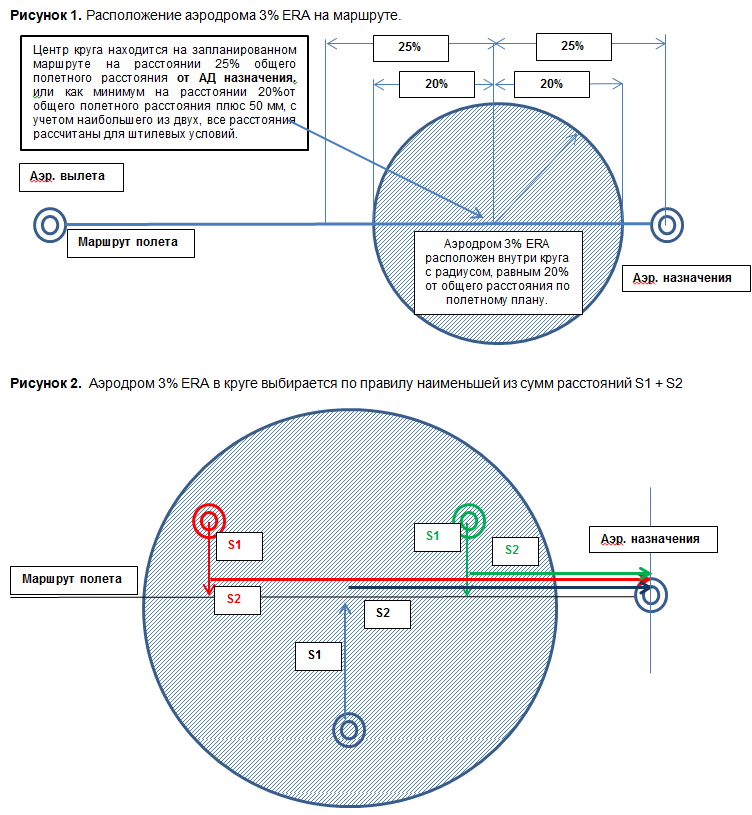
\includegraphics[width=0.9\linewidth]{Pictures/A8-ERAirdroms.png}
    \caption{}%\label{fig:ERA}    
\end{wrapfigure}
EXTRA ATC ALTERNATE – (в CFP как EXTRA – ATC) дополнительное топливо на полет в зоне ожидания запасного аэродрома. Определяется как топливо для полета в течение 5 минут на высоте 450 метров (1500f) в \textcolor[rgb]{1,0,0}{стандартных условиях и применяется для всех запасных аэродромов для исключения выхода экипажей в ситуацию, характеризующейся как «MINIMUM FUEL»} (\hyperref[par:1934]{пункте \ref*{par:1934}} данной главы) сообщением «PAN–PAN–PAN-MINIMUM FUEL.

Данный запас топлива не входит в расчет потребного количества топлива на полет для турбовинтовых ВС.

EXTRA WEATHER – (в CFP как EXTRA – WXX) дополнительное топливо на полет в зоне ожидания аэродрома назначения. Определяется как топливо для полета в течение 15 мин. на высоте 1500 м. (5000f) в стандартных условиях и применяется, если наступает один или несколько из перечисленных случаев: 
\begin{itemize}
    \item ко времени прилета прогнозируются временные изменения погоды (TEMPO) ниже минимума аэродрома пункта назначения;
    \item прогнозируемые ко времени прилета на аэродром назначения порывы ветра, превышают эксплуатационные ограничения;
    \item ко времени прилета прогнозируются сильные ливневые осадки, низкий коэффициент сцепления;
    \item ко времени прилета прогнозируются фронтальные грозы.
\end{itemize}


EXTRA DRIFTDOWN/DEPRESSURIZATION - (в CFP как EXTRA – DD/DP) дополнительное топливо для обеспечения возможности ВС выполнить при необходимости снижение и продолжить полет до запасного аэродрома при отказе двигателя или разгерметизации в наиболее критической точке на маршруте.

EXTRA RECLEARANCE - (в CFP как EXTRA – RECL) дополнительное топливо для полета с рубежа ухода на запасной. 

EXTRA FUEL ON BOARD (в CFP как EXTRA – FOB) топливо, которое оказалось на ВС в силу производственной необходимости или нештатной ситуации (замена ВС, отмена рейса и т.д.) при выполнении суточного плана полетов. 

\paragraph{} Во всех случаях окончательное решение о количестве топлива на борту принимает КВС на основании анализа метеорологической и аэронавигационной обстановки на маршруте, аэродромах вылета, назначения и запасных. 

\paragraph{} \label{par:497}Планирование и расположение запасного аэродрома по маршруту для уменьшения Contingency Fuel до 3\%.



\begin{enumerate}
    \item Планирование 3\% ERA представляет собой основанный на эксплуатационных характеристиках метод определения Contingency Fuel как запаса топлива в значении 3\% от запланированного количества топлива для полёта по маршруту, при соблюдении требований п. 4.3.6.3(c) и применения современных средств использования запасных аэродромов согласно п. 4.3.6.6 b(ii) части I Приложения 6 ИКАО,
    \item Назначение аэродрома 3\% ERA основывается на качественном и количественном допущении о том, что, даже если 3-процентный запас топлива на случай возникновения непредвиденных обстоятельств будет использован до достижения запланированного аэродрома назначения, на борту ВС будет оставаться достаточное количество топлива для выполнения посадки на этом аэродроме ERA с финальным резервом топлива.
    \item Расчет топлива с учетом местоположения аэродрома ERA не производится. Расположение аэродрома ERA позволяет выполнить безопасную посадку на нем, если уход на запасной аэродром осуществляется на крейсерском эшелоне во второй половине маршрута, но не далее точки TOD.
    \item Определение места и периода использования аэродрома 3\% ERA. 
    
    Аэродром 3\% ERA расположен внутри круга с радиусом, равным 20\% от общего расстояния по полетному плану, центр которого находится на запланированном маршруте на расстоянии 25\% общего полетного расстояния от АД назначения или, как минимум, на расстоянии 20\% от общего полетного расстояния плюс 50 nm, с учетом наибольшего из двух (см. \hyperref[fig:ERA]{рис. \ref*{fig:ERA}}); 

    \item Действия КВС в ситуации, когда полностью израсходован запас топлива на случай возникновения непредвиденных обстоятельств (плюс дополнительное количество топлива, взятое на борт по усмотрению КВС, если предусматривается) до достижения аэродрома назначения: 
    \begin{itemize}
        \item убедиться, что с учетом оставшихся дополнительных запасов топлива и тренда по топливу, остаток топлива над TOD будет не менее минимального количества топлива (указано в CFP), необходимого для продолжения полёта к аэродрому назначения;
        \item если расчеты и тренд по топливу продолжает оставаться отрицательным, рассмотреть возможность ухода на ближайший по маршруту пригодный запасной аэродром на маршруте, или на аэродром 3\% ERA; 
        \item в случае принятия решения ухода на аэродром 3\% ERA (точка изменения плана полета – любая точка маршрута, но не далее, чем точка маршрута TOD), выполните полет на него на крейсерском эшелоне, по кратчайшему расстоянию (по возможности «прямо на») используя запасные аэродромы на маршруте, которые были ранее определены в CFP, или запасные EDTO, если полет выполнялся по правилам EDTO.
    \end{itemize}
\end{enumerate} 

Во всех случаях величина дополнительного топлива ограничивается значениями эксплуатационных ограничений ВС в день выполнения полёта.

\begin{figure}[h]
    \centering    
    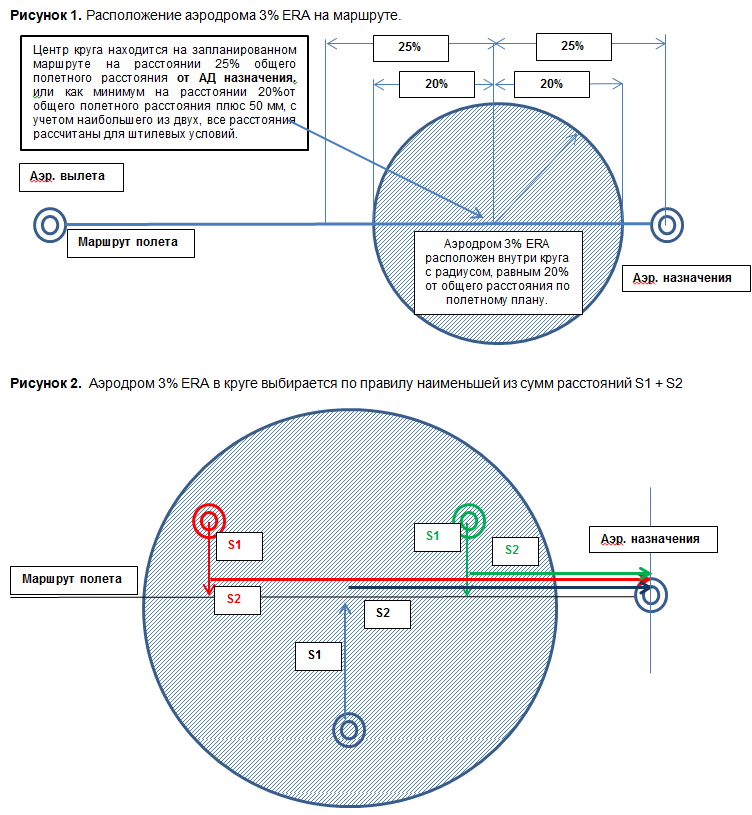
\includegraphics[width=0.6\linewidth]{Pictures/A8-ERAirdroms.png}
    \caption{}\label{fig:ERA}    
\end{figure}







\label{sec:visual}	Выполнение визуального захода на посадку


